\documentclass{article}

% if you need to pass options to natbib, use, e.g.:
%     \PassOptionsToPackage{numbers, compress}{natbib}
% before loading neurips_2021

% ready for submission
\usepackage[final]{neurips_2021}

% IMPORTANT: if you are submitting attention track, please add the attention option:
% \usepackage[attention]{neurips_2021}

% to compile a preprint version, e.g., for submission to arXiv, add add the
% [preprint] option:
%     \usepackage[preprint]{neurips_2021}

% to compile a camera-ready version, add the [final] option, e.g.:
% \usepackage[final]{neurips_2021}

% to avoid loading the natbib package, add option nonatbib:
%    \usepackage[nonatbib]{neurips_2021}

% \usepackage[utf8]{inputenc} % allow utf-8 input
% \usepackage[T1]{fontenc}    % use 8-bit T1 fonts
% \usepackage{hyperref}       % hyperlinks
% \usepackage{url}            % simple URL typesetting
% \usepackage{booktabs}       % professional-quality tables
% \usepackage{amsfonts}       % blackboard math symbols
% \usepackage{nicefrac}       % compact symbols for 1/2, etc.
% \usepackage{microtype}      % microtypography
% \usepackage{xcolor}         % colors
% \usepackage[authoryear]{natbib}
\usepackage[utf8]{inputenc} % allow utf-8 input
\usepackage[T1]{fontenc}    % use 8-bit T1 fonts
\usepackage{hyperref}       % hyperlinks
\usepackage{url}            % simple URL typesetting
\usepackage{booktabs}       % professional-quality tables
\usepackage{amsfonts}       % blackboard math symbols
\usepackage{nicefrac}       % compact symbols for 1/2, etc.
\usepackage{microtype}      % microtypography
\usepackage{xcolor}         % colors
\usepackage{graphicx}
\usepackage{amsmath}
\usepackage{float}
\usepackage{booktabs}
\usepackage{array}
\usepackage{makecell}
\usepackage{caption}
\usepackage{subcaption}
\captionsetup[figure]{skip=10pt} % Adjust the value as needed
\setlength{\bibsep}{0.0pt plus 0.2ex}

\title{Evaluating Uncertainty Quantification approaches for Neural PDEs in scientific application}

% Evaluating Uncertainty Quantification Approaches for Neural PDEs in Computational Fluid Dynamics 

% Neural PDEs-based Uncertainty Quantification Approaches for Computational Fluid Dynamics applications

% Neural PDEs-based Uncertainty Quantification Approaches for Scientific  applications

% The \author macro works with any number of authors. There are two commands
% used to separate the names and addresses of multiple authors: \And and \AND.
%
% Using \And between authors leaves it to LaTeX to determine where to break the
% lines. Using \AND forces a line break at that point. So, if LaTeX puts 3 of 4
% authors names on the first line, and the last on the second line, try using
% \AND instead of \And before the third author name.

% \author{%
%   Vardhan Dongre\\
%   % Department of Computer Science\\
%   University of Illinois Urbana-Champaign\\
%   Urbana, IL 61801 USA\\
%   \texttt{vdongre2@illinois.edu} \AND Gurpreet Singh Hora\\
%   % Department of Civil Engineering and Engineering Mechanics\\
%   Columbia University\\
%   New York, NY 10027 USA\\
%   \texttt{gh2546@columbia.edu}



% Author information can be set in various styles:
% For several authors from the same institution:
% \author{
% Vardhan Dongre \textsuperscript{1}\thanks{ \ \ vdongre2@illinois.edu}, \hspace{1mm} Gurpreet Singh Hora \textsuperscript{2} 
%  \\
%  \textsuperscript{1} University of Illinois Urbana-Champaign, \textsuperscript{2} Columbia University  
% \\
% }

\author{Vardhan Dongre\\ University of Illinois \\ \texttt{vdongre2@illinois.edu} \And Gurpreet Singh Hora \\ Columbia University\\ \texttt{gh2546@columbia.edu}}

  % examples of more authors
  % \And
  % Coauthor \\
  % Affiliation \\
  % Address \\
  % \texttt{email} \\
  % \AND
  % Coauthor \\
  % Affiliation \\
  % Address \\
  % \texttt{email} \\
  % \And
  % Coauthor \\
  % Affiliation \\
  % Address \\
  % \texttt{email} \\
  % \And
  % Coauthor \\
  % Affiliation \\
  % Address \\
  % \texttt{email} \\
% }
% \author{%
%   \begin{minipage}[t]{0.48\linewidth}
%     \centering
%     Vardhan Dongre\thanks{Use footnote for providing further information
%       about author (webpage, alternative address)---\emph{not} for acknowledging
%       funding agencies.} \\
%     Department of Computer Science\\
%     University of Illinois Urbana-Champaign\\
%     Urbana, IL 61801 USA\\
%     \texttt{\href{mailto:vdongre2@illinois.edu}{vdongre2@illinois.edu}}
%   \end{minipage}
%   \hfill
%   \begin{minipage}[t]{0.48\linewidth}
%     \centering
%     Gurpreet Singh Hora\\
%     Department of Civil Engineering and Engineering Mechanics\\
%     Columbia University\\
%     New York, NY 10027 USA\\
%     \texttt{\href{mailto:gh2546@columbia.edu}{gh2546@columbia.edu}}
%   \end{minipage}
% }

\begin{document}

\maketitle

\begin{abstract}
% With the increasing availability of geographically dispersed data, facilitated by affordable sensors, field experiments, numerical experiments, and satellite imagery, scientists now have a unique opportunity to tackle ongoing challenges within the field of climate change, weather prediction, and resilient urban development. 
% However, these sparse spatiotemporal measurements are limited in their ability to provide a comprehensive view of complex flow systems due to their relatively low sampling density.
% Neural Partial Differential Equations (PDEs), which combine deep learning (DL) techniques with domain expertise in PDE, boundary conditions, and initial conditions for parameterization, have demonstrated their effectiveness in capturing correlations within spatiotemporal datasets. 
% They excel at reconstructing a holistic understanding of flow systems based on partial measurements obtained from experiments and classical simulations of fluid dynamical systems. 
% Nevertheless, it's worth noting that the presence of noise in the data, coupled with the use of deep learning to approximate PDEs, introduces epistemic uncertainty.
% Therefore, a critical challenge lies in quantifying the uncertainties that propagate from the model inputs to the outputs, particularly when dealing with noisy measurements. This is essential for establishing the reliability and trustworthiness of predictive models.
% This research is dedicated to evaluating various Uncertainty Quantification (UQ) approaches, which are crucial for both forward and inverse problems in scientific applications. Specifically, we investigate the effectiveness of Bayesian methods, such as Hamiltonian Monte Carlo (HMC) and Monte-Carlo Dropout (MCD), and a more conventional approach, Deep Ensembles (DE), in quantifying uncertainties. 
% To illustrate their performance, we apply these approaches to two examples: Burger's equation and the Navier-Stokes equation.
% Our findings indicate that both approaches accurately reconstruct flow systems and predict the associated parameters. 
% Additionally, we observed that Bayesian methods tend to produce results that exhibit a higher degree of confidence compared to the traditional DE method.

% Scientific computations in computational fluid dynamics (CFD) have often grappled with the formidable challenges posed by inverse and ill-posed problems arising from incomplete data, uncertain initial and boundary conditions, and the omnipresent specter of sensor noise. Deep learning-based methods combined with non-linear partial differential terms for parameterization have shown effectiveness in capturing correlations within the spatiotemporal datasets obtained from simulations of fluid dynamical systems. However, the quantification of uncertainties propagated from model inputs to outputs remains a challenge and an important goal for establishing the trustworthiness of these predictions. This work focuses on assessing various Uncertainty Quantification (UQ) approaches essential for both Forward and Inverse scientific problems and their utility for the propagation of uncertainty in computational models. In particular, we take two practical examples from CFD and their canonical partial differential equations to examine the efficacy of Hamiltonian Monte Carlo (HMC), Monte-Carlo Dropout (MCD), and the Deep Ensembles (DE) methods.

The accessibility of spatially distributed data, enabled by affordable sensors, field, and numerical experiments, has facilitated the development of data-driven solutions for scientific problems, including climate change, weather prediction, and urban planning. Neural Partial Differential Equations (Neural PDEs), which combine deep learning (DL) techniques with domain expertise (e.g., governing equations) for parameterization, have proven to be effective in capturing valuable correlations within spatiotemporal datasets. However, sparse and noisy measurements coupled with modeling approximation introduce aleatoric and epistemic uncertainties. Therefore, quantifying uncertainties propagated from model inputs to outputs remains a challenge and an essential goal for establishing the trustworthiness of Neural PDEs. This work evaluates various Uncertainty Quantification (UQ) approaches for both Forward and Inverse Problems in scientific applications. Specifically, we investigate the effectiveness of Bayesian methods, such as Hamiltonian Monte Carlo (HMC) and Monte-Carlo Dropout (MCD), and a more conventional approach, Deep Ensembles (DE). To illustrate their performance, we take two canonical PDEs: Burger's equation and the Navier-Stokes equation. Our results indicate that Neural PDEs can effectively reconstruct flow systems and predict the associated unknown parameters. However, it is noteworthy that the results derived from Bayesian methods, based on our observations, tend to display a higher degree of certainty in their predictions as compared to those obtained using the DE. This elevated certainty in predictions suggests that Bayesian techniques might underestimate the true underlying uncertainty, thereby appearing more confident in their predictions than the DE approach.
\end{abstract}

\section{Introduction}

% For scientific computations, it has been observed that classical numerical methods are not only computationally expensive but also intractable for challenging inverse and ill-posed problems. These challenges may arise due to sparse and noisy measurements, incomplete material properties, and unknown initial and boundary conditions. 

% As an alternative, Deep Learning based approaches provided promising solutions however they suffer from physical inconsistencies. Physics Informed Neural Networks (PINNs) that combined domain knowledge with observed/simulated data are able to tackle these challenges at much faster computational speeds. bpi

While conventional Deep Learning-based approaches provide promising avenues for the scientific domain, they often struggle to uphold the physical realizability of the solutions. Physics-Informed Neural Networks (PINNs), as introduced by \citep{raissi2019physics}, excel at incorporating soft physical constraints within the neural network optimization process, leading to better outcomes. However, due to noisy and limited data, the accuracy of these models can degrade significantly. Adopting these methods, in principle, requires the models and their predictions to be reliable, due to which our ability to quantify the uncertainties involved in the process becomes significantly valuable.

% in developing reliable ML methods for scientific problems.

The UQ problem has two intimately coupled components \citep{najm2009uncertainty}. The first pertains to the forward propagation of uncertainty from model parameters to model outputs, and the second component involves the estimation of the parametric uncertainties themselves based on available data. The focus of this work is to quantify the total uncertainty from both components. The task of UQ in scientific machine learning is complex, given the stochastic processes in science, model overparameterization, and data noise \citep[e.g.,][]{he2023survey, gal2016uncertainty, basu2022uncertainty, zou2022neuraluq}. Past research has employed diverse Bayesian and Deterministic strategies to quantify model uncertainty, but a comparative understanding of these methods’ efficacy remains elusive. This study seeks to fill this gap by systematically comparing various uncertainty quantification techniques, including Hamiltonian Monte Carlo (HMC), Monte Carlo Dropouts (MCD), and Deep Ensembles (DE).
We apply these methods to forward and inverse problems in two canonical PDEs - the Burger’s equation and the Navier-Stokes equation, illustrating their performance in reconstructing flow systems and predicting parameters from sparse noisy measurements. 
% \textbf{You can remove the conclusion from introduction ``Notably, .....}
% Notably, our observations suggest that predictions derived from Bayesian methods exhibit higher certainty than those from DE. This difference raises the possibility that Bayesian techniques might underestimate the true underlying uncertainty, appearing overly confident in their predictions compared to DE approaches. Future work should investigate this apparent discrepancy in predictive certainty between Bayesian and DE methods to ensure more accurate uncertainty quantification in scientific machine learning applications.

%  \textbf{DL models can suffer from
% physical inconsistencies or yield implausible predictions due to
% data biases (67). PINNs aim at addressing this challenge by
% incorporating fundamental physical symmetries and domain
% knowledge into the DL architecture and loss function. This
% approach constrains the model to satisfy physics constraints in
% addition to observations, thereby improving its performance
% and robustness (76).}

% UQ in scientific machine learning presents a challenging problem due to various factors such as the stochastic nature of scientific processes, model overparameterization, and data noise. While several works \cite{} have attempted to quantify model uncertainty using different Bayesian and Deterministic strategies, there is no clear understanding of the benefits of using one method over the other in terms of their performance, data requirements, and computational demands. This study aims to systematically compare different methods to quantify model uncertainties. The approaches considered in this work include Hamiltonian Monte Carlo (HMC), Variational Inference (VI), Monte Carlo Dropouts (MCD), and Deep Ensembles (DE) in both forward and inverse problems.


\section{Forward Problems}
% In scientific problems, PDEs represent a governing relationship between certain parameters or variables.
Consider a parameterized and non-linear PDE that characterizes the behavior of a physical system, defined as 
\begin{equation}
    \mathbf{\mathcal{L}}_{\mathbf{x}}[\mathbf{u};\mathbf{\lambda}] = \mathbf{f} (\mathbf{x},t),  \mathbf{x} \in \Omega,  t \in [0, T],
\end{equation}
where $\mathbf{u}(\mathbf{x},t)$ denotes the latent state (aka solution field), the $\mathbf{\mathcal{L}}_{\mathbf{x}}[.;\mathbf{\lambda}]$ is a general differential operator parameterized by $\mathbf{\lambda}$, $\mathbf{f} (\mathbf{x},t)$ is the forcing term which refers to any external influences on the system, while $\Omega \subset \mathbb{R}^{D}$ is the bounded domain in a d-dimensional physical space.

Given this framework and noisy measurements of $\mathbf{u}(\mathbf{x},t), \mathbf{f} (\mathbf{x},t)$, the goal is to infer the latent state $\mathbf{u}( \mathbf{x},t)$ of the dynamical system. In forward problems, PINNs as well as their Bayesian variants B-PINNs are typically used as surrogates 
$\widetilde{\mathbf{u}}(\mathbf{x}, t; \mathbf{\theta})$, to infer either point estimates or posterior distributions of this latent state. In the Bayesian framework, the parameters $\theta$ of the surrogates have a prior distribution $P(\mathbf{\theta})$ and its formulation is defined as: 
\begin{equation}
    \widetilde{\mathbf{f}}(\mathbf{x}, t; \mathbf{\theta}) := \mathbf{\mathcal{L}}_{\mathbf{x}} [\widetilde{\mathbf{u}}(\mathbf{x}, t; \mathbf{\theta});\mathbf{\lambda}]
\end{equation}
$P(\mathcal{D}|\mathbf{\theta})$ represents the likelihood while the Bayes' Theorem estimates the final posterior distribution. 
\begin{equation}
    p(\mathbf{\theta} | \mathcal{D}) = \frac{P(\mathcal{D}|\mathbf{\theta})P(\mathbf{\theta})}{P(\mathcal{D})} \cong P(\mathcal{D}|\mathbf{\theta})P(\mathbf{\theta})
\end{equation}

% For brevity of notation, unnecessary indicates are omitted from $\mathbf{u}$ and $\mathbf{f}$ for the further sections.
\vspace{-0.15cm}
To approximate the posterior distribution, we employ both Bayesian methods like HMC and MCD as well as deterministic DE approach. HMC is an efficient Markov Chain Monte Carlo (MCMC) sampling method that uses concepts from Hamiltonian Dynamics and utilizes momentum variables to guide the proposals in the Markov chain, which can lead to faster convergence and better exploration of the target distribution. Given the continuous nature of Hamiltonian dynamics, leapfrog integration is used as a numerical technique to discretize and update the momentum and position variables in a staggered manner over discrete time steps. In our Bayesian methodology, we posit an independent Gaussian distribution as the prior $P(\mathbf{\theta})$. For HMC, parameters for Burger's (Navier-Stokes) equation include a leapfrog step of 50 (50), an initial time step of 0.1 (0.01), 1000 (5000) burn-in steps, and a sampling size of 100 (100). With DE, we assemble an ensemble of PINNs equivalent in number to the HMC samples, set at 100 (200). For MCD, we induce variance by sporadically dropping neurons at a 1\% (1\%) dropout rate during each training iteration. To gauge prediction uncertainty, we execute 100 (200) inferences with HMC. For DE, we acquire 100 (200) predictions from each ensemble member, and for MCD, we undertake forward network propagation 100 (200) times, maintaining the established dropout rate.
% VI on the other hand turns the problem into an optimization problem and estimates the target distribution by minimizing the KL divergence between the approximation and the true posterior. In the Bayesian approaches we have assumed an independent Gaussian distribution for the prior $P(\mathbf{\theta})$. For HMC we set the leapfrog step size to be \textbf{val}, the initial time step as \textbf{val}, number of burn-in steps as \textbf{val}, and the number of samples to be \textbf{val}. For DE we construct an ensemble of PINNs, with \textbf{val} members same as the number of samples obtained from HMC, and for MCD we randomly drop a certain number of neurons using a dropout rate of \textbf{val} at each training step. To estimate the uncertainty around predictions we perform \textbf{val} inferences using HMC, for DE we obtain \textbf{val} predictions from each member and we run the forward propagation of network \textbf{val} times with the same dropout rate for MCD.  

\subsection{1-D Burger’s Equation}
Burger's equation is a PDE that arises in fluid dynamics and represents a combination of diffusion and convection processes.
It has wide applications in various scientific domains, including traffic flow modeling \citep{nagatani2000density}, acoustics and sound propagation \citep{naugolnykh2000nonlinear}, and material transport in porous media \citep{shah2016solution}.
% It describes the behavior of a fluid flow in one dimension and includes both advection and diffusion terms. The equation is typically written as:
% Burger's equation is a fundamental non-linear partial differential equation representing a combination of diffusion and convection processes.
For this work, we consider a one-dimensional Burger's equation with Dirichlet boundary condition and sinusoidal initial conditions:
\begin{equation}
\frac{\partial u}{\partial t} + u \cdot \nabla u  - \frac{0.01}{\pi} \nabla^2 u = 0, ~~ x \in [-1,1], ~ t\in [0,1],
\end{equation} 
\vspace{-0.65cm}
\begin{gather*}
    u(0,x) = - sin(\pi x), \\
    u(t,-1) = u(t,1) = 0,
\end{gather*}
where $x$ represents the spatial location, $t$ represents time, $u (x,t)$ represents the velocity of the fluid, and $\nabla$ and $\nabla^2$ represents gradient and Laplacian operators.
% This equation arises in various areas of applied mathematics, including fluid mechanics, nonlinear
% acoustics, gas dynamics, and traffic flow [14].

To find its exact solution, we employ the Chebfun package \citep{rico1994continuous}, utilizing spectral Fourier discretization with 512 modes and a fourth-order explicit Runge-Kutta temporal integrator featuring a time step of $\Delta t=10^{-6}$. 
 For a more comprehensive understanding, consult the methodology detailed in \citep{raissi2019physics}.
Here, we operate under the assumption that the exact solution remains unknown.
Instead, we rely on noisy sensors that capture 2000 spatiotemporal readings for $u$ and $f$. 
The noise in these measurements adheres to a Gaussian distribution with scales $\epsilon_f \sim \mathcal{N}(0, 0.1^2)$ and $\epsilon_u \sim \mathcal{N}(0, 0.1^2)$. 
In our experiments, we employ a multilayer perceptron (MLP) neural network consisting of eight hidden layers, each comprising 20 neurons with tanh non-linearity.
%
\begin{figure}[H]
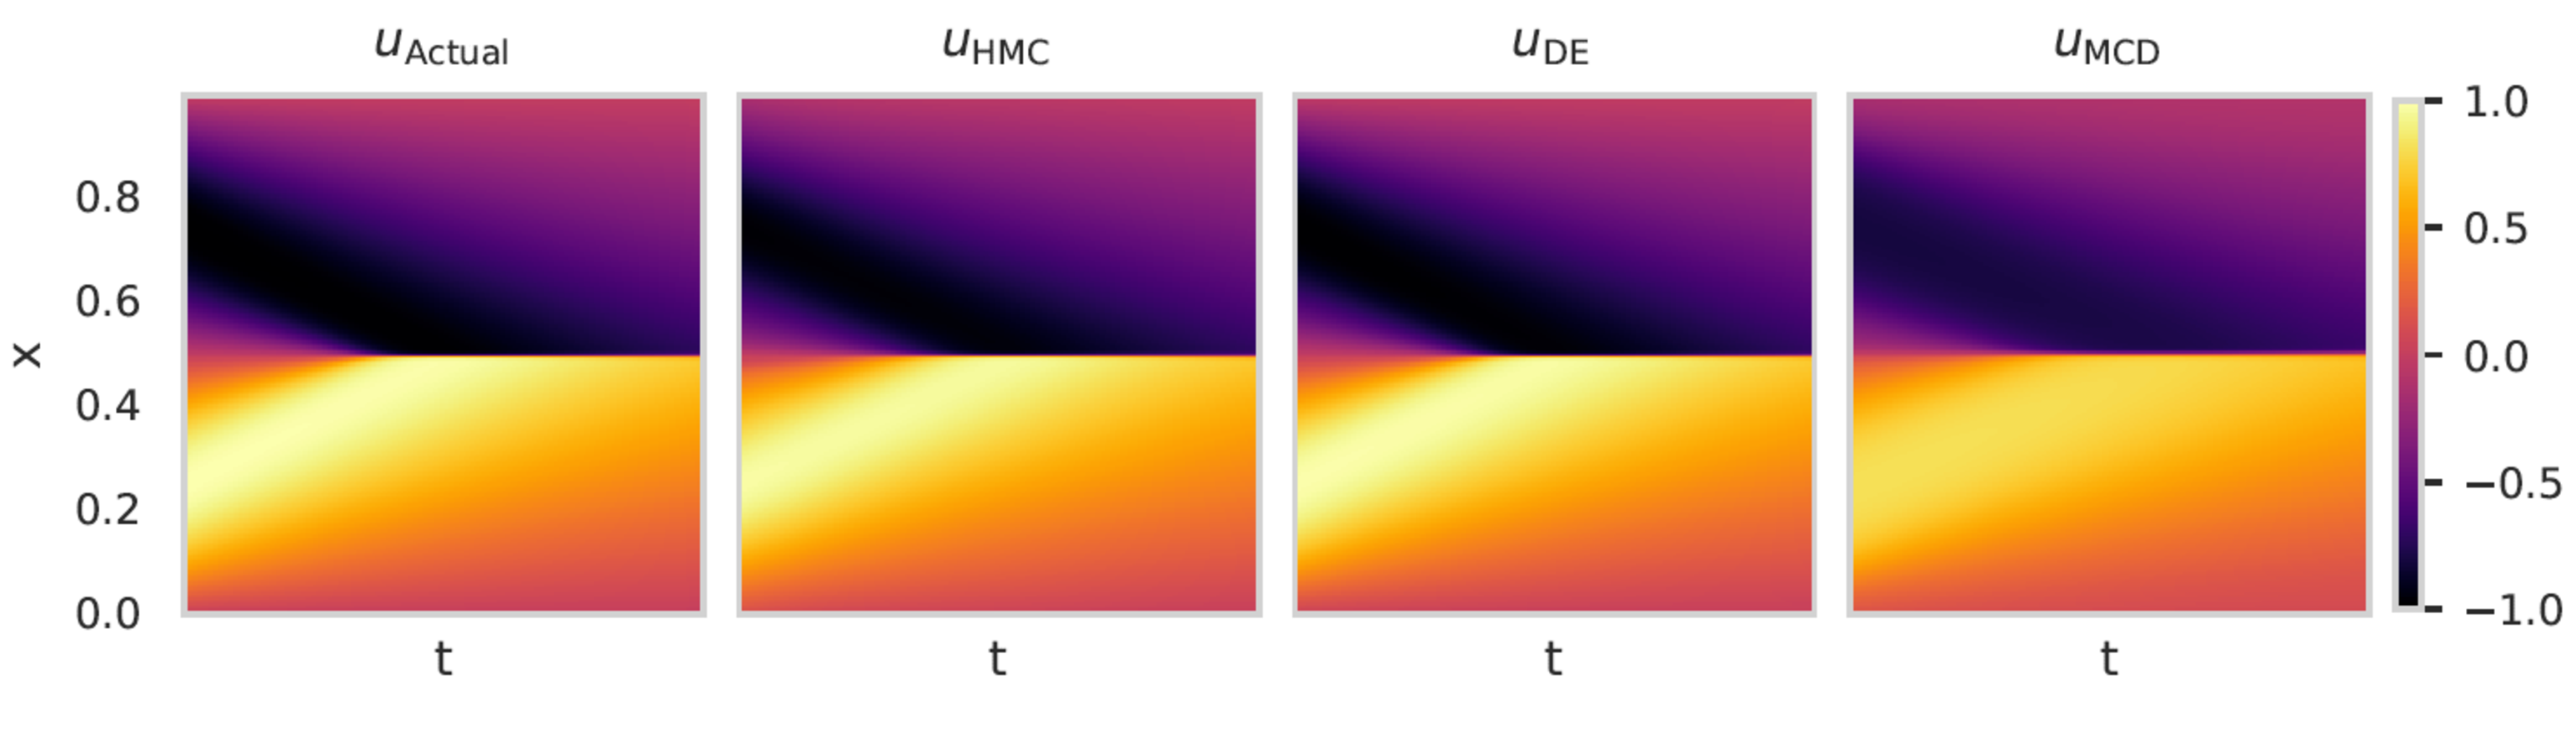
\includegraphics[width=\linewidth]{images/Burgers_velocity_comparision_23_1.pdf}
\caption{One-dimensional Burgers equation - forward problem: comparison of the spatiotemporal evolution of predictive mean and exact solutions for $u$. HMC represents Hamiltonian Monte Carlo, DE represents Deep Ensembles, MCD represents Monte Carlo Dropout, and Actual represents the exact solution.}
\label{fig:heat-map}
\end{figure}
%
Figure \ref{fig:heat-map} presents a comparative analysis of predictive spatiotemporal means derived from three distinct approaches, juxtaposed against the reference actual solution, denoted as ($u_{\mathrm{Actual}}$).
An initial visual assessment of these predictions reveals their impressive fidelity to the exact solutions, effectively reconstructing the solution to the Burgers equation in both space and time from sparse measurements.
Notably, within Figure \ref{fig:heat-map}, it becomes evident that both the HMC ($u_{\mathrm{HMC}}$) and DE ($u_{\mathrm{DE}}$) approaches provide accurate predictions of the magnitude of $u$, closely matching the actual solution. In contrast, the MCD ($u_{\mathrm{MCD}}$) consistently underestimates the magnitude of the solution.

%
\begin{figure}
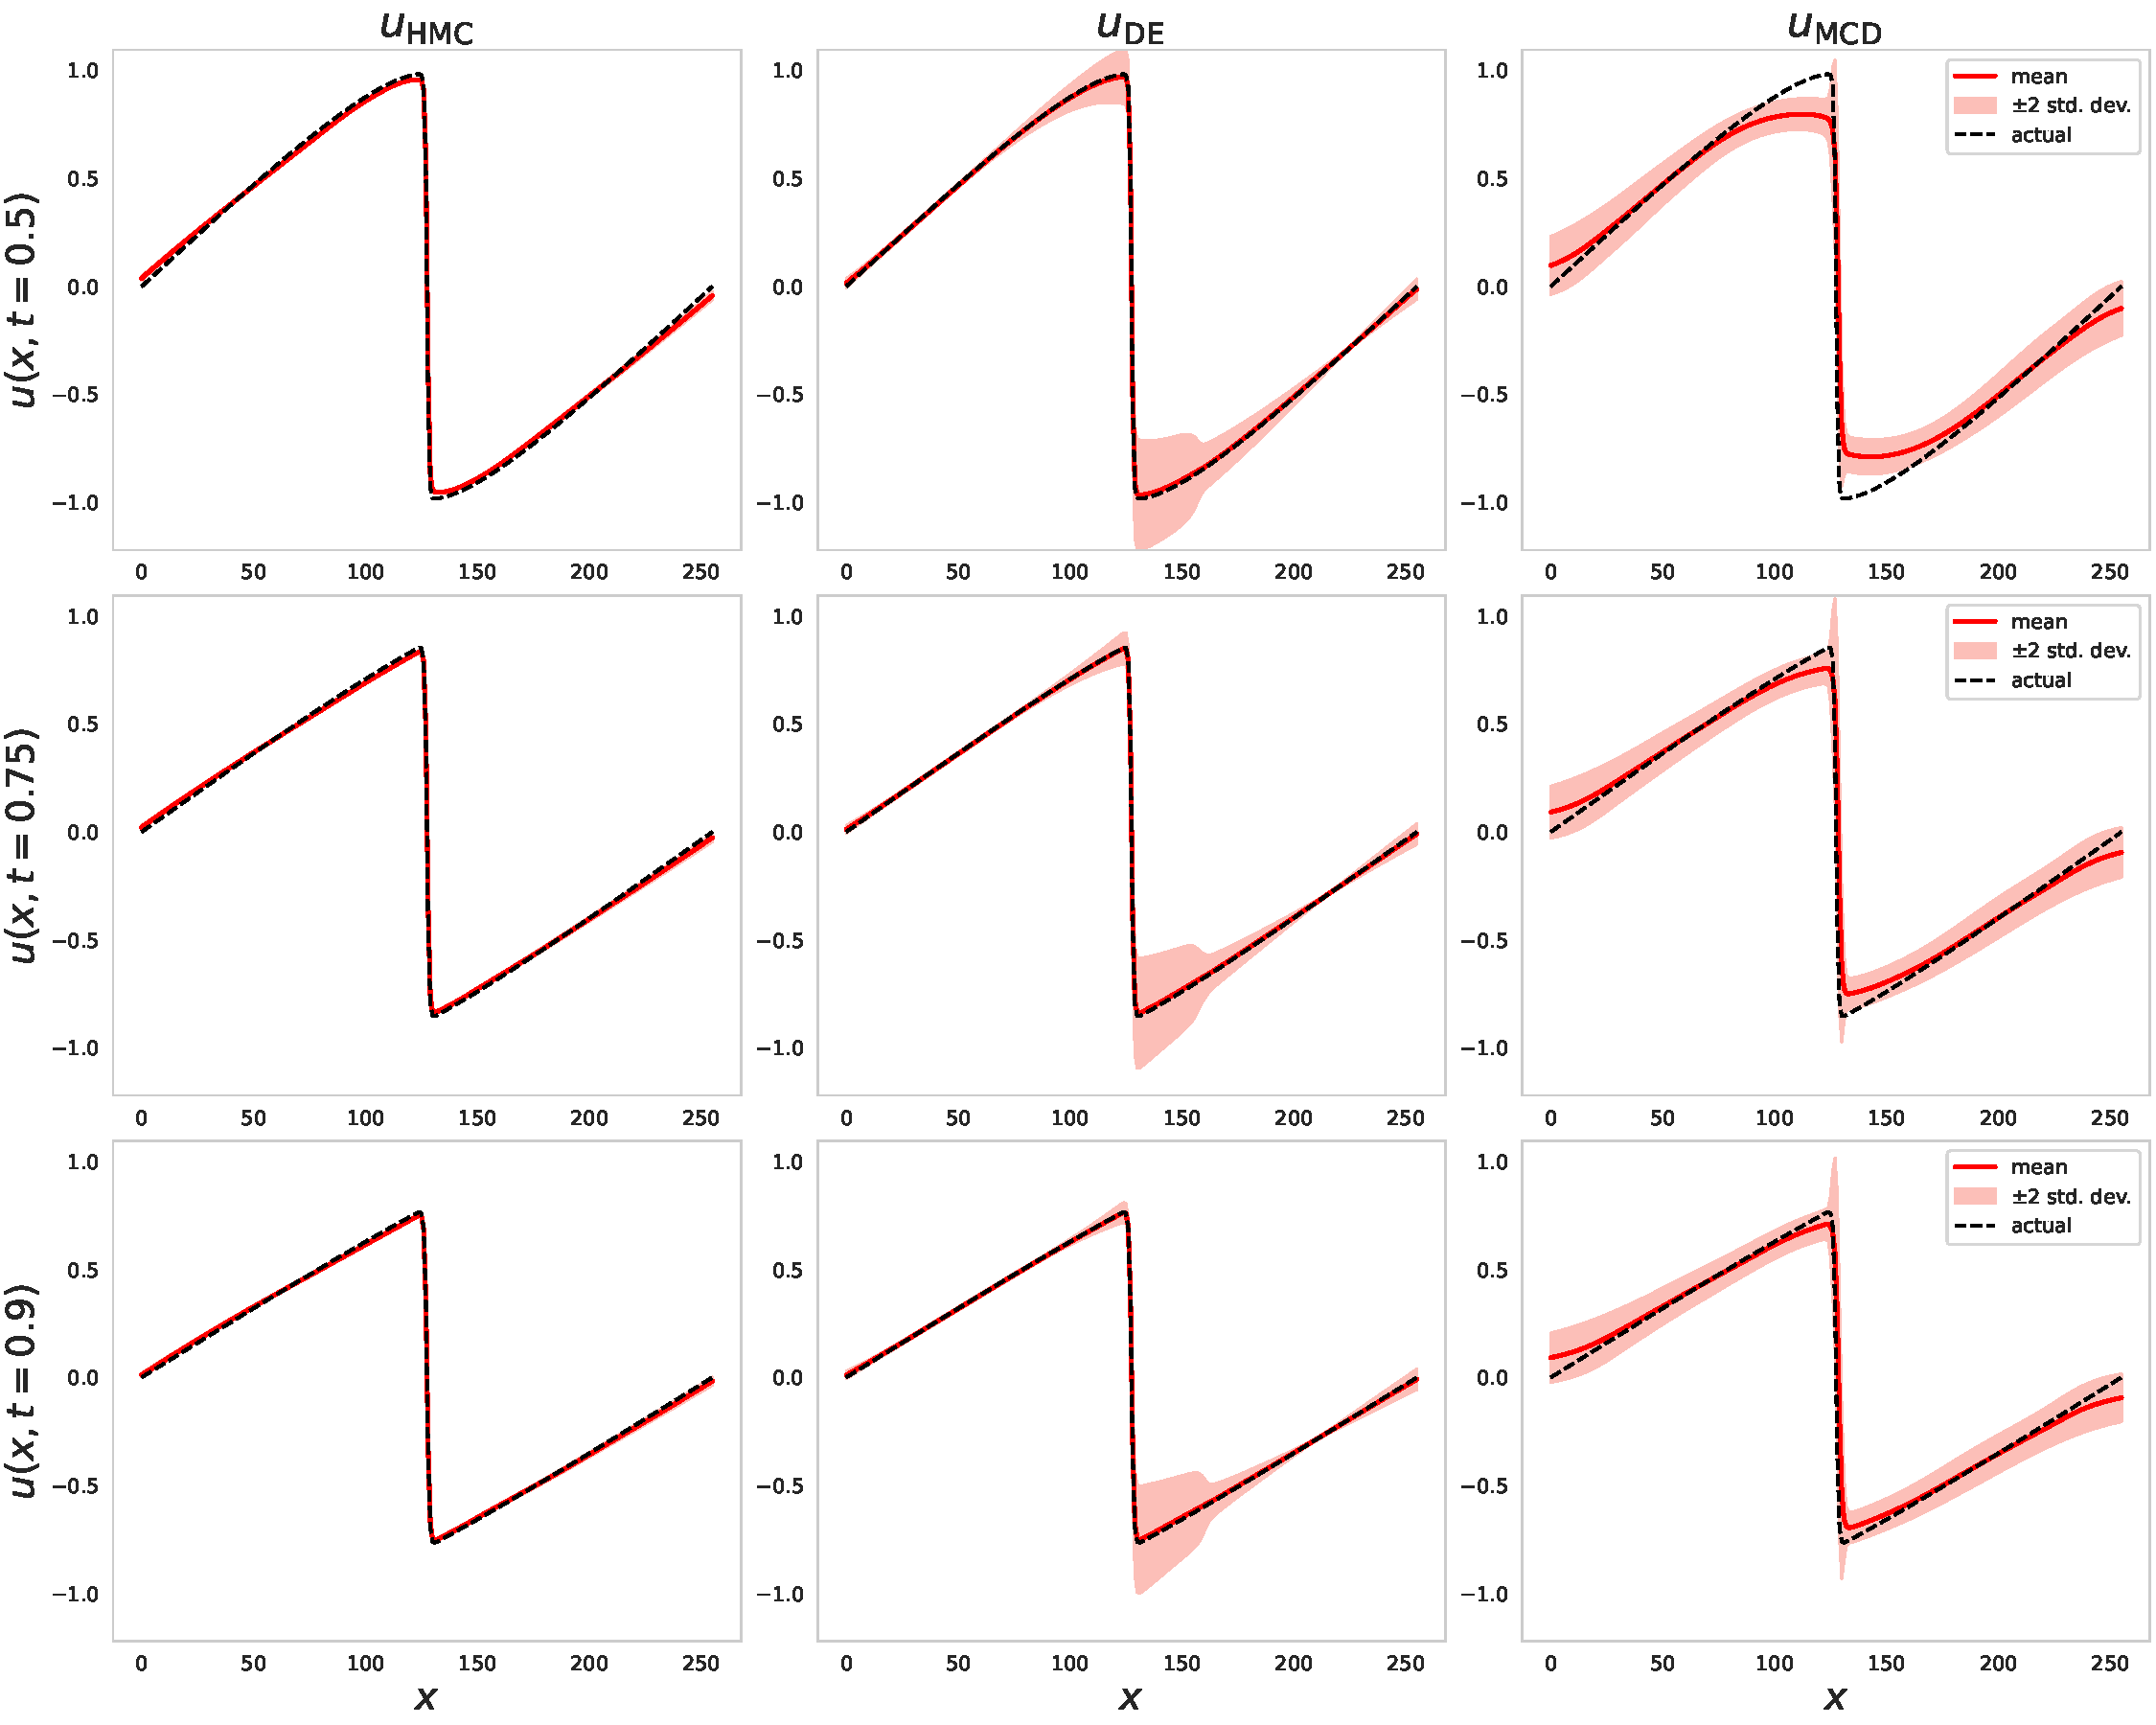
\includegraphics[width=\linewidth]{images/Burgers_1d_comparison-5.pdf}
\caption{One-dimensional Burgers equation - forward problem: comparison of the predicted and exact solutions corresponding to the three temporal snapshots denoted by $t \in \{0.50s, 0.75s, 0.90s\}$ from different methods.}
\label{fig:1D-comparision}
\end{figure}
%
The spatiotemporal color maps of the predictive mean do not effectively convey the model's confidence in its predictive capabilities.
To investigate the uncertainties in the predictions, the predictive means along with the corresponding two standard deviation confidence intervals generated by three different methods, HMC, MCD, and DE, for the variable $u$ at three distinct time snapshots, namely, $t = 0.50s, 0.75s, 0.90s$ are illustrated in figure  \ref{fig:1D-comparision}.
From visual inspection, it is evident that both the HMC and DE approaches provide reasonably accurate posterior estimations of the variable $u$ at all three time-snapshots. 
Moreover, the error between these predictive means and the actual solution remains predominantly within the bounds of the two standard deviations.
In contrast, the MCD approach exhibits discrepancies from the actual solution across all temporal snapshots, although these discrepancies tend to diminish as time progresses. 
It is noteworthy that, for $t = 0.50s$, a significant portion of the error falls outside the two standard deviation confidence intervals.
However, as time advances, the performance of the MCD approach noticeably improves. It is also important to highlight that all three approaches effectively capture the formation of shocks, a challenging task even for classical numerical methods.

Our results show that the Bayesian approaches, i.e., HMC render overconfident results while model outputs from DE and MCD are appropriately conservative as expected \citep{basu2022uncertainty}.
In conclusion, both HMC and DE seem to be superior in terms of both prediction accuracy and uncertainty quantification, especially when compared to the results from MCD. 
While MCD's performance improves with time, its initial underestimation of uncertainty could be problematic, especially in scenarios where early-stage predictions are critical.

\subsection{2-D Navier Stokes Equation}\label{sec:NS-eqn}
Our next example delves into a practical scenario involving the flow of an incompressible fluid, a phenomenon elegantly described by the renowned Navier-Stokes equations. 
These equations stand as a cornerstone in the realm of scientific and engineering dynamics, offering profound insights and applications. 
They find utility in several geophysical and engineering domains, such as climate prediction \citep{palmer2019stochastic}, air pollution \citep{adair2015reynolds}, aerodynamics of aircraft and cars \citep{hassan2014numerical, liu2016navier, vos2002navier}, and blood circulation \citep{thomas2016blood, AlbertoS}. 
% Beyond these, the Navier-Stokes equations can aid in the study of blood circulation, the assessment of pollutant dispersion, and a myriad of other scientific and engineering endeavors. 
In this work, we consider a prototype problem of incompressible flow past a cylinder, and the governing equation can be defined as follows:
%
\begin{equation}\label{eqn:NS}
    \frac{\partial \mathbf{u}}{\partial t} + \lambda_1 \mathbf{u} \cdot \nabla \mathbf{u} + \nabla \mathbf{u} - \lambda_2 \nabla^2 u = 0, \\
     % \nabla \cdot \mathbf{u} = 0
\end{equation}
\begin{gather*}
    \nabla \cdot \mathbf{u} = 0,
\end{gather*}
%

% ~~ \Omega \in [-15, 25] \times [-8, 8] \times [0,10] 
where $\mathbf{u}=\{u,v\}$ represents the velocity in $x$ and $y$ direction, $p$ represents the pressure of the fluid, $t$ represent time, and $\mathbf{\lambda}=\{\lambda_1, \lambda_2\}$ are the parameters and for the forward problems $\lambda_1$ is set to 1 and $\lambda_2$ to $10^{-2}$.
Given the multidimensional nature of this problem, it offers a challenging testbed for the Bayesian approach to quantify uncertainties in both the velocity and pressure fields.
It is important to emphasize that pressure measurements are not included in the model training; instead, the neural network predicts them based on the governing equation. To generate the exact solutions, we leverage the data provided for the work by \citep{raissi2019physics}, and readers are advised to refer to the same for more details.

Similarly, we operate under the assumption that the precise solution remains elusive while our sensors diligently capture 5000 spatiotemporal readings for both $u$ and $f$.
These measurements exhibit a Gaussian distribution with scales $\epsilon_f \sim \mathcal{N}(0, 0.1^2)$ and $\epsilon_u \sim \mathcal{N}(0, 0.1^2)$. 
To effectively approximate the latent variables in the Navier-Stokes equation—namely, $u$, $v$, and $p$ -- we employ an MLP network comprising ten hidden layers, each housing 20 neurons with a tanh non-linearity.

%
\begin{figure}
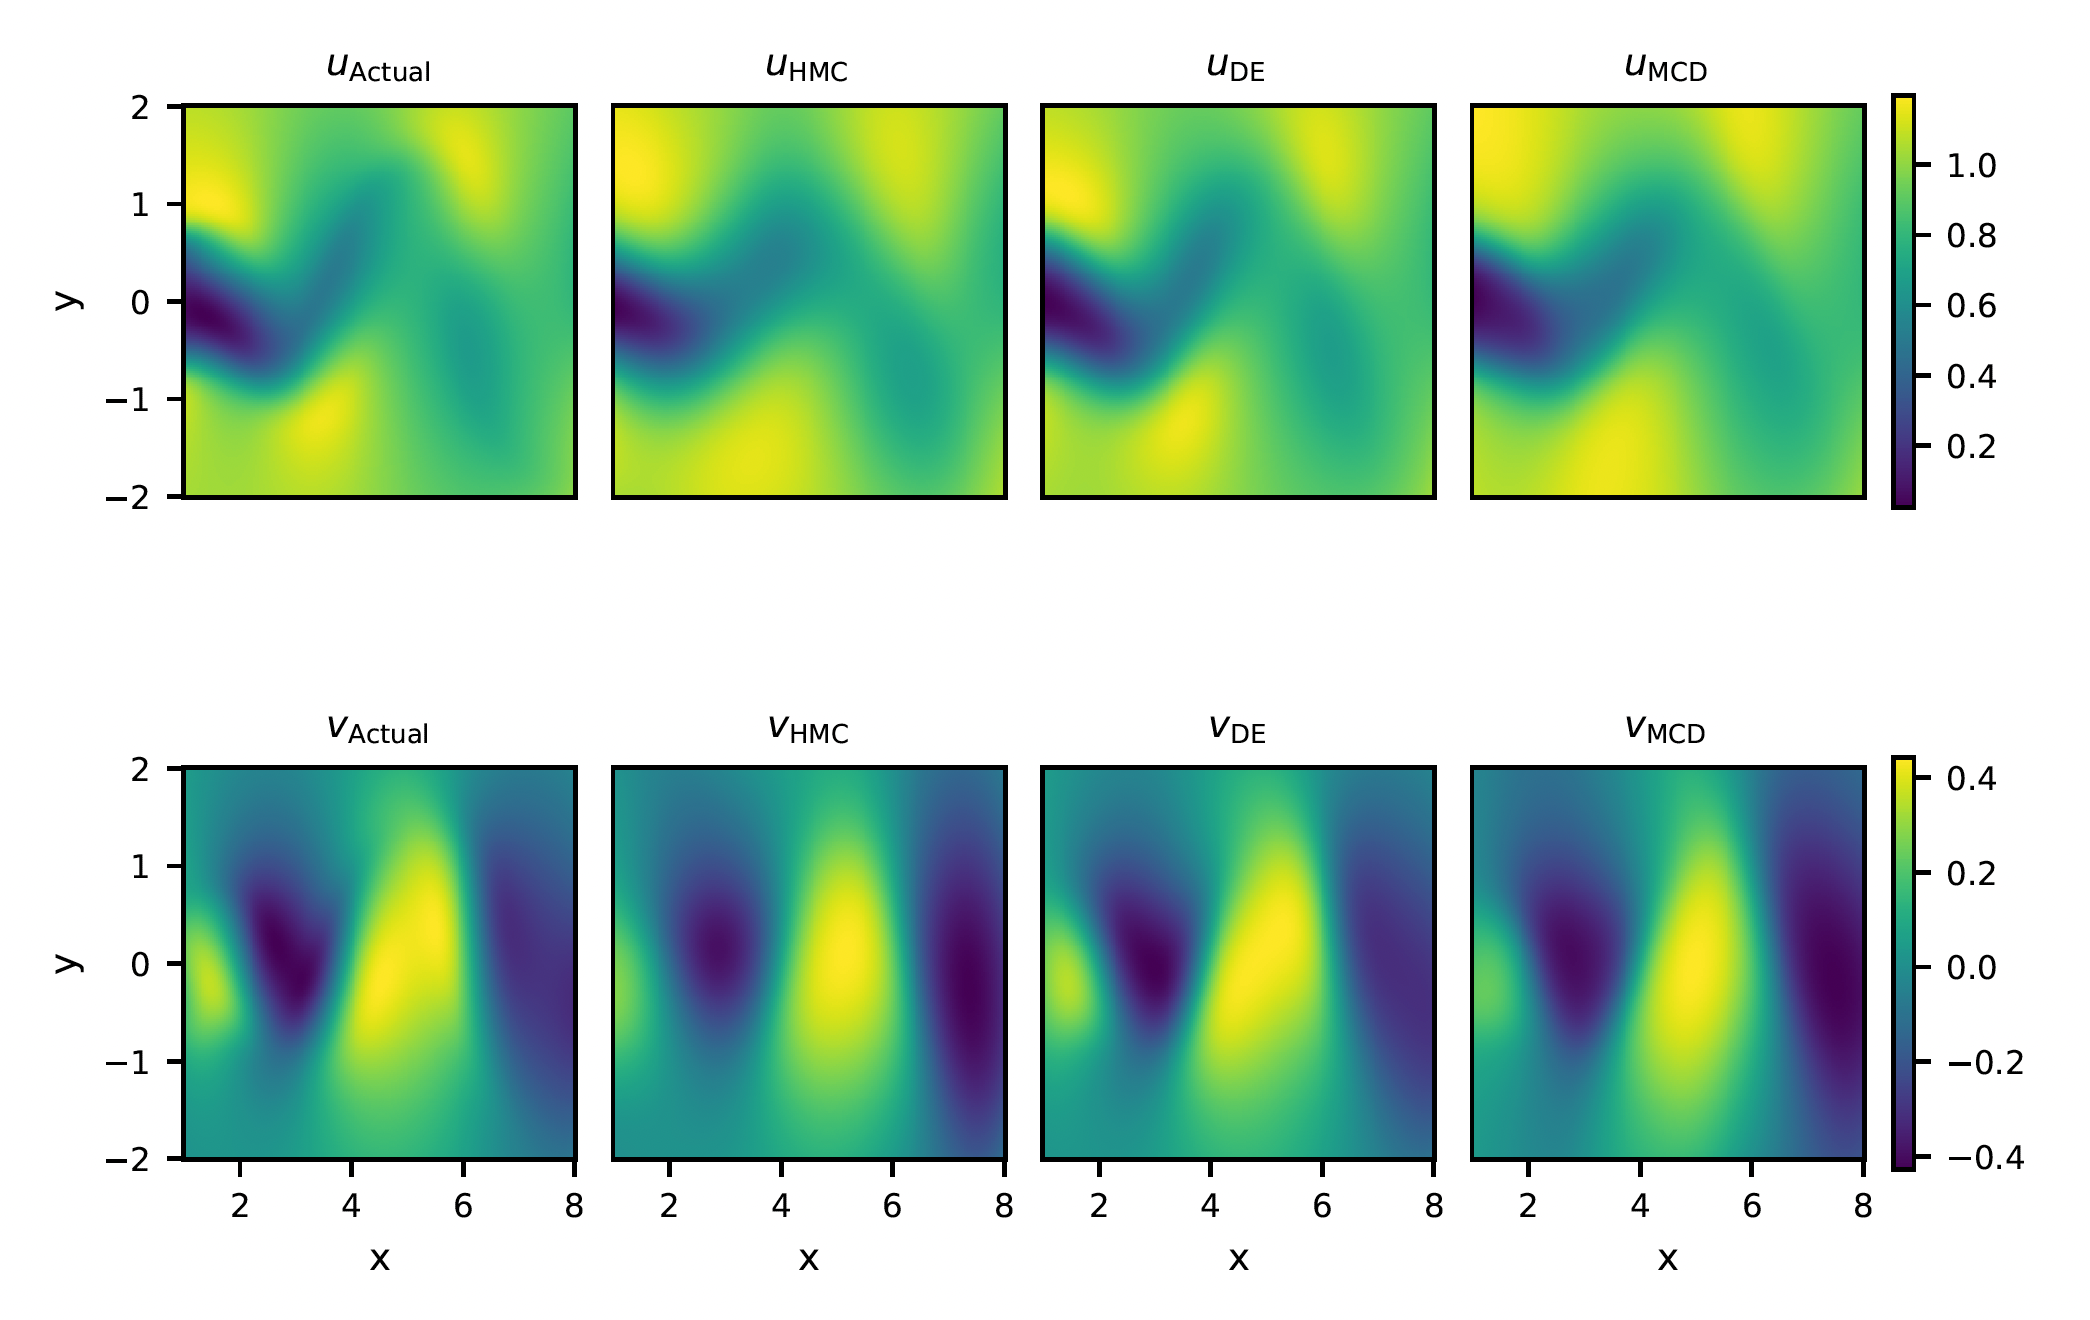
\includegraphics[width=\linewidth]{images/NSforward.png}
\caption{Navier-Stokes equation - forward problem: Instantaneous predictive mean for velocity component in $x$-direction $u$ (top) and $y$-direction $v$ (bottom) using HMC, DE, and MCD approaches is compared against the actual instantaneous $u$ and $v$ components at a representative time instant.}
\label{fig:navier-stokes-mean}
\end{figure}
%

The predictive means obtained from HMC, DE, and MCD for the velocity components $u$ and $v$ are compared with the reference actual solution, figure \ref{fig:navier-stokes-mean}. 
It is readily apparent from the figure that all three models have adeptly reconstructed the $u$ and $v$ velocity components. 
This remarkable accuracy is achieved despite the challenges posed by the noisy, scattered sensor data across the entire spatiotemporal domain.
Moreover, we examine the $\mathrm{L}_1$ norm-based error between the actual and predictive mean values to gain further insights, as presented in figure \ref{fig:navier-stokes-error}.
Notably, the DE approach exhibits the closest agreement with the actual solutions. 
In contrast, the error for the HMC and MCD approaches is roughly three times higher than that observed with the DE approach for both velocity components.
Importantly, it is worth noting that, across all proposed methodologies, the errors consistently remain within the bounds of two standard deviations, as illustrated in figure \ref{fig:navier-stokes-sigma}.
This observation underscores our confidence in the predictions generated by these various approaches, as they remain well within the established confidence interval.
%
\begin{figure}
    \centering
    \vspace{-20mm}
    \begin{subfigure}[b]{\linewidth}
        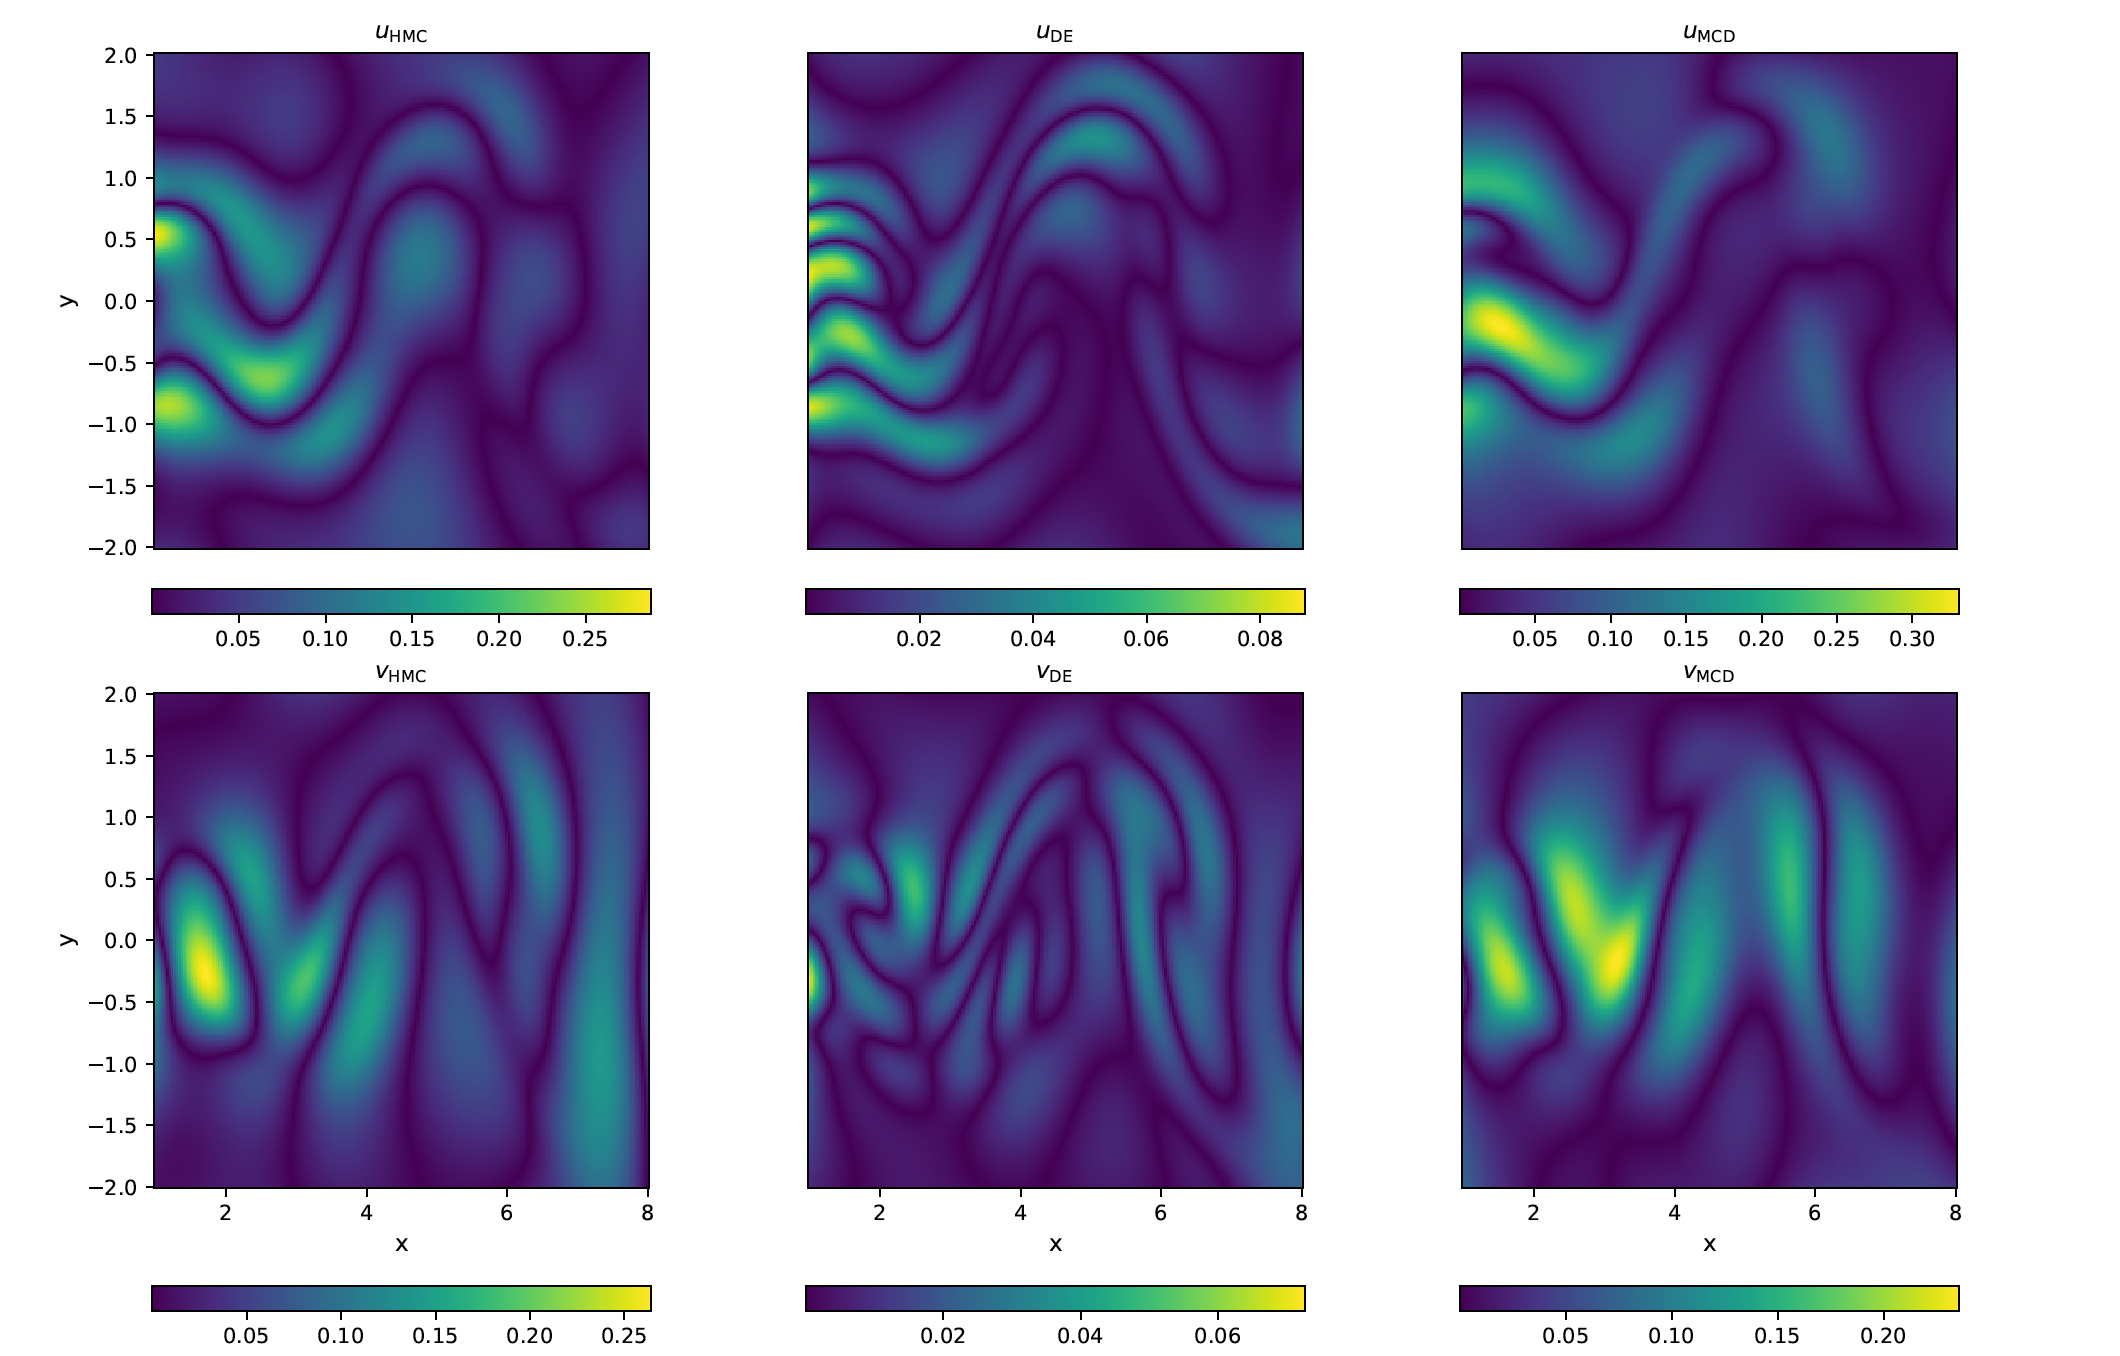
\includegraphics[width=\linewidth, keepaspectratio]{images/1.png}
        \caption{Predictive errors for velocity component in $x$-direction $u$ (top) and $y$-direction $v$ (bottom) from different methods at a representative time instant.}
        \label{fig:navier-stokes-error}
    \end{subfigure}
    \vspace{1em} % Adjust the space as needed
    \begin{subfigure}[b]{\linewidth}
        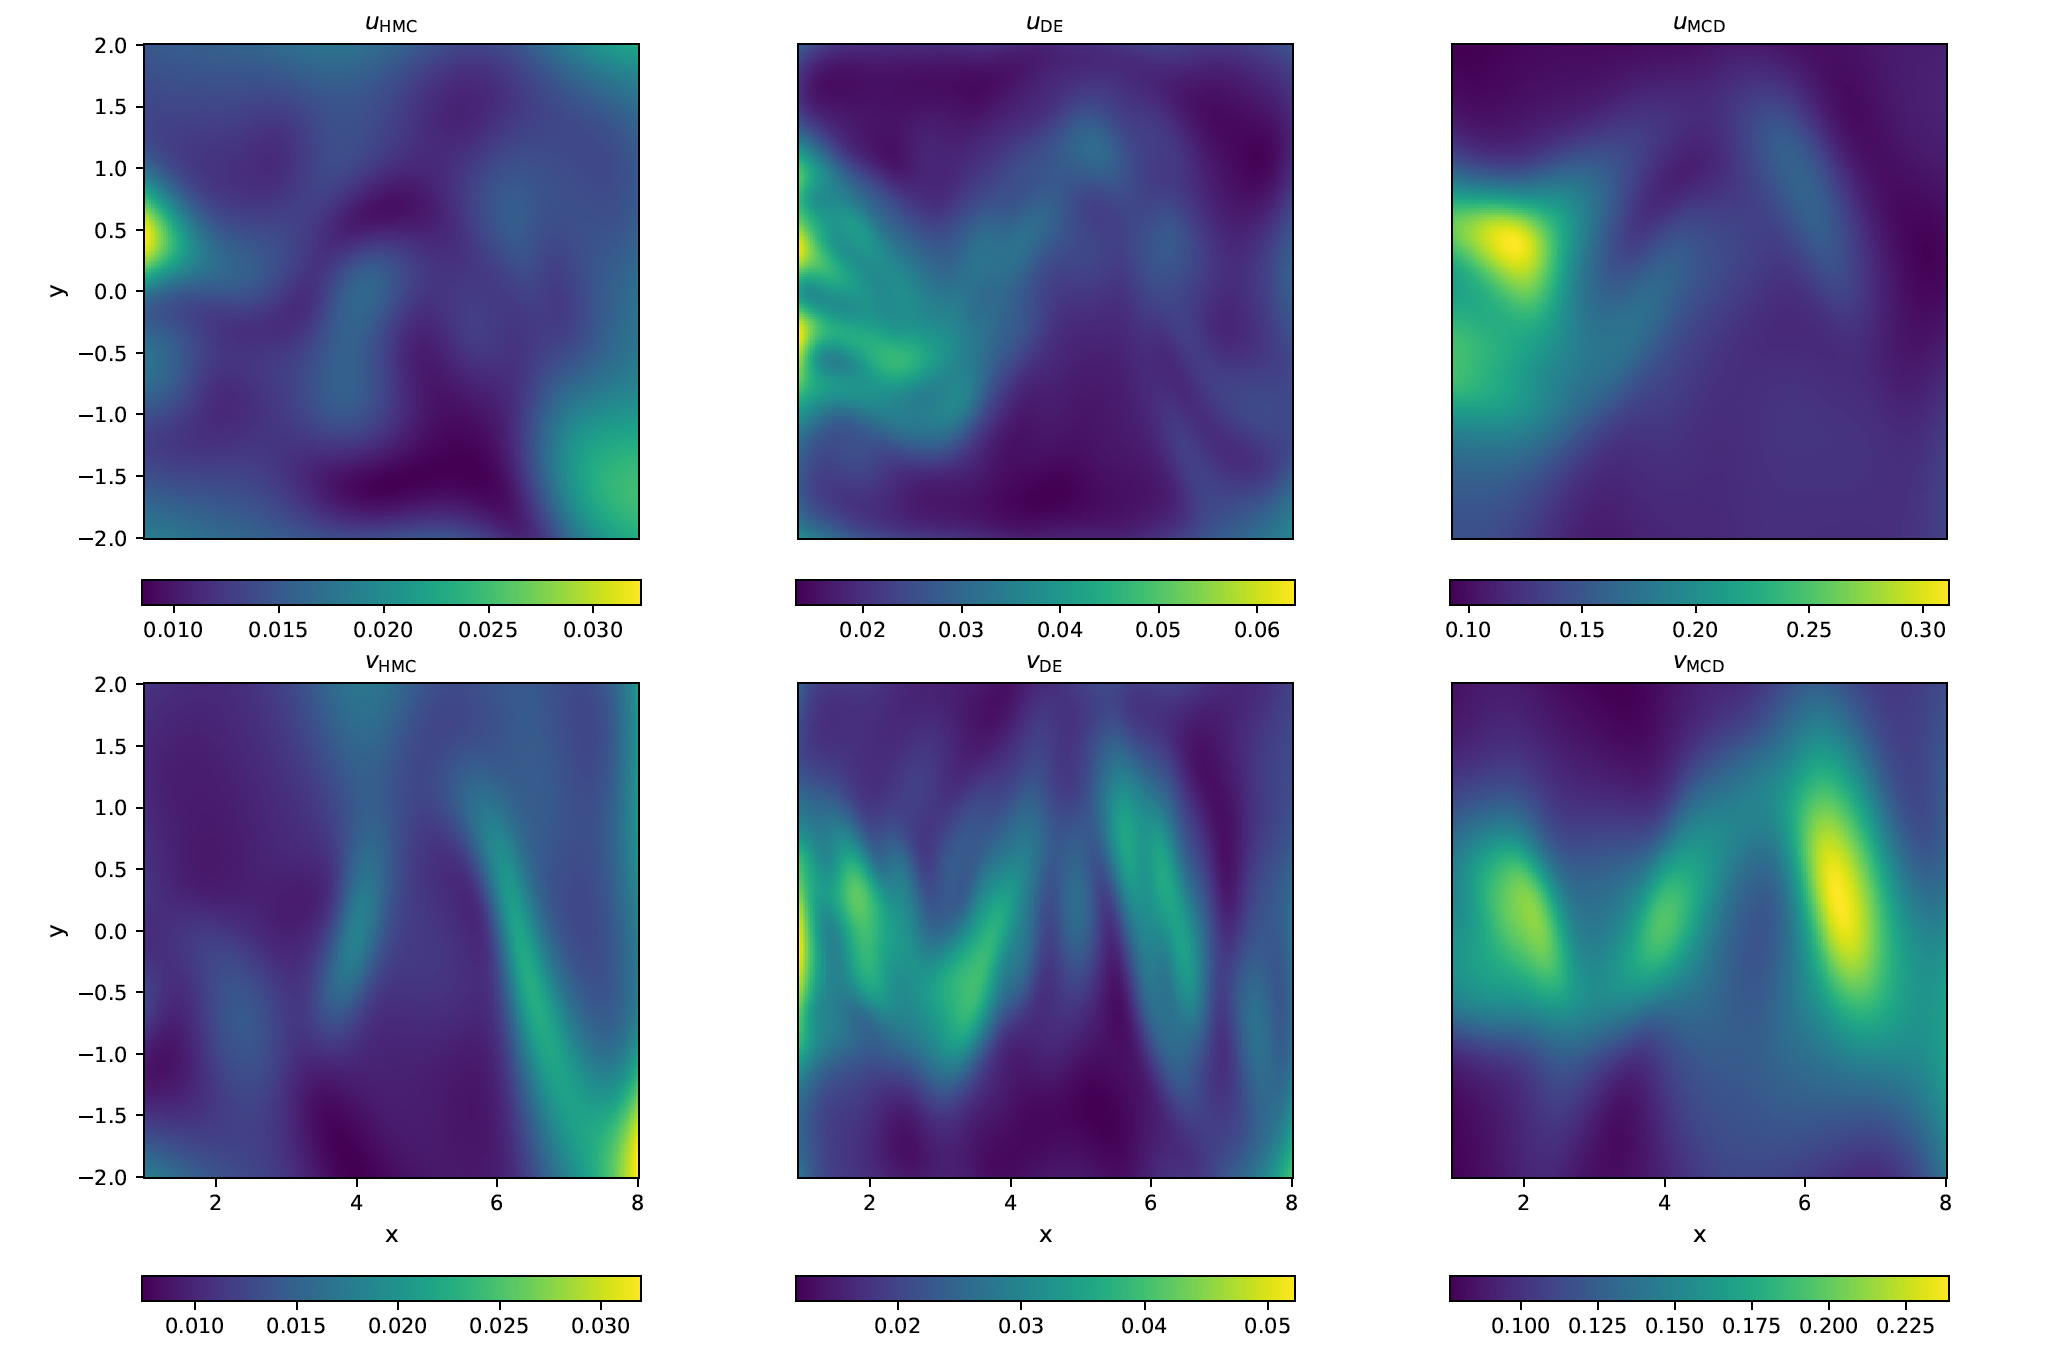
\includegraphics[width=\linewidth, keepaspectratio]{images/2.png}
        \caption{Two standard deviations $(\sigma)$ for velocity component in $x$-direction $u$ (top) and $y$-direction $v$ (bottom) from different methods at a representative time instant.}
        \label{fig:navier-stokes-sigma}
    \end{subfigure}
    \caption{Navier-Stokes equation - forward problem.}
\end{figure}

% \begin{figure}
% \includegraphics[width=0.8\linewidth, keepaspectratio]{images/NS_velocity_error_comparison.pdf}
% \caption{Navier-Stokes equation - forward problem: Predictive errors for velocity component in $x$-direction $u$ (top) and $y$-direction $v$ (bottom) from different methods at a representative time instant.}
% \label{fig:navier-stokes-error}
% \end{figure}
% \vspace{-10em} % Adjust this value as needed to reduce space between figures

% \begin{figure}
% \includegraphics[width=0.8\linewidth, keepaspectratio]{images/NS_velocity_std_comparison.pdf}
% \caption{Navier-Stokes equation - forward problem: Two standard deviations $(\sigma)$ for velocity component in $x$-direction $u$ (top) and $y$-direction $v$ (bottom) from different methods at a representative time instant.}
% \label{fig:navier-stokes-sigma}
% \end{figure}

% \begin{figure}
% \includegraphics[width=0.8\linewidth, keepaspectratio]{images/NS_velocity_error_comparison.pdf}
% \caption{Navier-Stokes equation - forward problem: Predictive errors for velocity component in $x$-direction $u$ (top) and $y$-direction $v$ (bottom) from different methods at a representative time instant.}
% \label{fig:navier-stokes-error}
% \end{figure}


% %
% \begin{figure}
% \includegraphics[width=0.8\linewidth, keepaspectratio]
% % \includegraphics[width=\linewidth, height=4cm]
% {images/NS_velocity_std_comparison.pdf}
% \caption{Navier-Stokes equation - forward problem: Two standard deviations $(\sigma)$ for velocity component in $x$-direction $u$ (top) and $y$-direction $v$ (bottom) from different methods at a representative time instant.}
% \label{fig:navier-stokes-sigma}
% \end{figure}
%
% Some ideas for conclusion/introduction
% The deterministic PINNs approach, as demonstrated in previous work \citep{raissi2019physics}, has shown its capability to reconstruct velocity components from sparse spatiotemporal measurements. 
% However, what sets the approaches considered in this paper apart is their ability not only to reconstruct velocity components accurately but also to provide associated uncertainties.
% These uncertainties play a pivotal role in assessing the model's robustness, allowing us to make well-informed decisions regarding the deployment of machine learning models in real-world scenarios, for instance, weather prediction. 
% They serve as a crucial tool in gauging the reliability and confidence we can place in the model's predictions, enhancing our ability to navigate practical applications with greater certainty.

\section{Inverse Problems}

Inverse problems involve determining a system's underlying parameters $\mathbf{\lambda}$ and physical properties from observable data. 
% This often entails identifying coefficients or boundary conditions that lead to observed states for PDEs.

In the context of our study, B-PINN offers a systematic approach to tackle inverse problems. We can quantify uncertainties in the estimated parameters by propagating uncertainties through the network and leveraging the Bayesian framework. Similar to the framework described in equations [2-3], apart from a surrogate for $\theta$, we also assign a prior distribution for $\lambda$, which can be independent of the prior for $\theta$. The likelihood is then defined as $P(\mathcal{D}|\theta, \lambda)$, and we then calculate the joint posterior of $[\theta, \lambda]$:
\begin{equation}
    p(\theta, \lambda | \mathcal{D}) = \frac{P(\mathcal{D}|\theta, \lambda)P(\theta, \lambda)}{P(\mathcal{D})} \cong P(\mathcal{D}|\theta, \lambda)P(\theta, \lambda) = P(\mathcal{D}|\theta, \lambda)P(\theta)P(\lambda)
\end{equation}
%
%
\newcolumntype{V}[1]{>{\centering\arraybackslash}m{#1}|}
%
\captionsetup[table]{skip=15pt}
\begin{table}[ht]
  \centering
  \begin{tabular}{V{3cm}c c c}
    \toprule[2pt]  % Thicker top horizontal line
     & HMC & DE & MCD \\
    \midrule  % Regular middle horizontal line
    $\lambda_{1}$ (mean $\pm$ std) & \makecell{$0.758$ $\pm$ $0.0$} & \makecell{$0.957$ $\pm$ $0.024$} & \makecell{$0.843$ $\pm$ $0.075$} \\
    $\lambda_{2}$ (mean $\pm$ std) & \makecell{$0.017$ $\pm$ $2.13\mathrm{e}{-06}$} & \makecell{$0.014$ $\pm$ $0.001$} & \makecell{$0.015$ $\pm$ $0.058$} \\
    \bottomrule[2pt]  % Thicker bottom horizontal line
  \end{tabular}
  \caption{Navier Stokes equation - inverse problem : Predictions for $\lambda_{1}, \lambda_{2}$ using HMC, DE, MCD; actual values for $\lambda_{1} = 1.0, \lambda_{2} = 0.01$}
  \label{tab:inverse}
\end{table}
%
% \begin{figure}
%     \centering
%     \includegraphics[scale=0.5\linewidth]{images/Burgers_1d_comparison.pdf}
%     \caption{Enter Caption}
%     \label{fig:enter-label}
% \end{figure}
The PDE considered for the inverse problem is the same Navier-Stokes equation (Refer equation \ref{eqn:NS}).
However, in the context of the inverse problems, the parameters $\lambda= \{\lambda_1, \lambda_2\}$ are now considered unknown.
The primary objective here is to identify the values of unknown parameters based on the limited measurements of $f$ and $\mathbf{u}=[u,v]$ outlined in section \ref{sec:NS-eqn}.

The MLP model we employ for the inverse problem has ten hidden layers with 40 neurons in each layer and tanh non-linearity.
The predicted values of $\lambda$ from considered approaches are displayed in Table \ref{tab:inverse}.
The DE method has provided relatively precise estimates, reflecting a good degree of certainty in its predictions. This suggests that ensemble techniques effectively capture these parameters’ underlying distributions. While HMC provides high confidence in its estimates, the absence of uncertainty is unrealistic, and this overconfidence could be a sign of the model not capturing all sources of uncertainty. MCD provides a broader uncertainty estimation, which might be capturing more sources of uncertainties, but it could also be overestimating the uncertainty in the parameters. The wider confidence intervals for MCD could either mean that MCD is being more cautious or it’s not as effective in pinpointing the true parameter values.
% Conversely, the HMC and MCD approaches feature larger errors compared to DE.
% Moreover, HMC, in particular, displays an inherent overconfidence in its predictions, consistent with our expectations.
These findings underscore the effectiveness of the DE approach in not only identifying the unknown parameters but also quantifying the uncertainty arising from the sparse and noisy sensor measurements.


\section{Summary}
This research comparatively evaluates various UQ approaches, with particular emphasis on Bayesian methods and the Deep Ensemble (DE) technique. While all approaches, including DE, HMC, MCD, effectively reconstruct flow systems for the two examples considered, Bayesian methods demonstrate higher certainty in predictions but may underestimate the total uncertainty, thereby appearing overly confident. In contrast, while offering more conservative certainty estimates, the DE method is computationally more demanding. We also acknowledge that the performance of these methods improves by inferring more samples, but due to computational constraints, we restrict the numbers to 100 (200) for Burger's (Navier Stokes) Equation. The study underscores the need for balancing predictive certainty, computational efficiency, and accuracy when using Bayesian or DE approaches for flow system modeling and parameter prediction. 
% \section{General formatting instructions}
% \label{gen_inst}


% The text must be confined within a rectangle 5.5~inches (33~picas) wide and
% 9~inches (54~picas) long. The left margin is 1.5~inch (9~picas).  Use 10~point
% type with a vertical spacing (leading) of 11~points.  Times New Roman is the
% preferred typeface throughout, and will be selected for you by default.
% Paragraphs are separated by \nicefrac{1}{2}~line space (5.5 points), with no
% indentation.


% The paper title should be 17~point, initial caps/lower case, bold, centered
% between two horizontal rules. The top rule should be 4~points thick and the
% bottom rule should be 1~point thick. Allow \nicefrac{1}{4}~inch space above and
% below the title to rules. All pages should start at 1~inch (6~picas) from the
% top of the page.


% For the final version, authors' names are set in boldface, and each name is
% centered above the corresponding address. The lead author's name is to be listed
% first (left-most), and the co-authors' names (if different address) are set to
% follow. If there is only one co-author, list both author and co-author side by
% side.


% Please pay special attention to the instructions in Section \ref{others}
% regarding figures, tables, acknowledgments, and references.


% \section{Headings: first level}
% \label{headings}


% All headings should be lower case (except for first word and proper nouns),
% flush left, and bold.


% First-level headings should be in 12-point type.


% \subsection{Headings: second level}


% Second-level headings should be in 10-point type.


% \subsubsection{Headings: third level}


% Third-level headings should be in 10-point type.


% \paragraph{Paragraphs}


% There is also a \verb+\paragraph+ command available, which sets the heading in
% bold, flush left, and inline with the text, with the heading followed by 1\,em
% of space.


% \section{Citations, figures, tables, references}
% \label{others}


% These instructions apply to everyone.


% \subsection{Citations within the text}


% The \verb+natbib+ package will be loaded for you by default.  Citations may be
% author/year or numeric, as long as you maintain internal consistency.  As to the
% format of the references themselves, any style is acceptable as long as it is
% used consistently.


% The documentation for \verb+natbib+ may be found at
% \begin{center}
%   \url{http://mirrors.ctan.org/macros/latex/contrib/natbib/natnotes.pdf}
% \end{center}
% Of note is the command \verb+\citept+, which produces citations appropriate for
% use in inline text.  For example,
% \begin{verbatim}
%    \citept{hasselmo} investigated\dots
% \end{verbatim}
% produces
% \begin{quote}
%   Hasselmo, et al.\ (1995) investigated\dots
% \end{quote}


% If you wish to load the \verb+natbib+ package with options, you may add the
% following before loading the \verb+neurips_2023+ package:
% \begin{verbatim}
%    \PassOptionsToPackage{options}{natbib}
% \end{verbatim}


% If \verb+natbib+ clashes with another package you load, you can add the optional
% argument \verb+nonatbib+ when loading the style file:
% \begin{verbatim}
%    \usepackage[nonatbib]{neurips_2023}
% \end{verbatim}


% As submission is double blind, refer to your own published work in the third
% person. That is, use ``In the previous work of Jones et al.\ [4],'' not ``In our
% previous work [4].'' If you cite your other papers that are not widely available
% (e.g., a journal paper under review), use anonymous author names in the
% citation, e.g., an author of the form ``A.\ Anonymous'' and include a copy of the anonymized paper in the supplementary material.


% \subsection{Footnotes}


% Footnotes should be used sparingly.  If you do require a footnote, indicate
% footnotes with a number\footnote{Sample of the first footnote.} in the
% text. Place the footnotes at the bottom of the page on which they appear.
% Precede the footnote with a horizontal rule of 2~inches (12~picas).


% Note that footnotes are properly typeset \emph{after} punctuation
% marks.\footnote{As in this example.}


% \subsection{Figures}


% \begin{figure}
%   \centering
%   \fbox{\rule[-.5cm]{0cm}{4cm} \rule[-.5cm]{4cm}{0cm}}
%   \caption{Sample figure caption.}
% \end{figure}


% All artwork must be neat, clean, and legible. Lines should be dark enough for
% purposes of reproduction. The figure number and caption always appear after the
% figure. Place one line space before the figure caption and one line space after
% the figure. The figure caption should be lower case (except for first word and
% proper nouns); figures are numbered consecutively.


% You may use color figures.  However, it is best for the figure captions and the
% paper body to be legible if the paper is printed in either black/white or in
% color.


% \subsection{Tables}


% All tables must be centered, neat, clean and legible.  The table number and
% title always appear before the table.  See Table~\ref{sample-table}.


% Place one line space before the table title, one line space after the
% table title, and one line space after the table. The table title must
% be lower case (except for first word and proper nouns); tables are
% numbered consecutively.


% Note that publication-quality tables \emph{do not contain vertical rules.} We
% strongly suggest the use of the \verb+booktabs+ package, which allows for
% typesetting high-quality, professional tables:
% \begin{center}
%   \url{https://www.ctan.org/pkg/booktabs}
% \end{center}
% This package was used to typeset Table~\ref{sample-table}.


% \begin{table}
%   \caption{Sample table title}
%   \label{sample-table}
%   \centering
%   \begin{tabular}{lll}
%     \toprule
%     \multicolumn{2}{c}{Part}                   \\
%     \cmidrule(r){1-2}
%     Name     & Description     & Size ($\mu$m) \\
%     \midrule
%     Dendrite & Input terminal  & $\sim$100     \\
%     Axon     & Output terminal & $\sim$10      \\
%     Soma     & Cell body       & up to $10^6$  \\
%     \bottomrule
%   \end{tabular}
% \end{table}

% \subsection{Math}
% Note that display math in bare TeX commands will not create correct line numbers for submission. Please use LaTeX (or AMSTeX) commands for unnumbered display math. (You really shouldn't be using \$\$ anyway; see \url{https://tex.stackexchange.com/questions/503/why-is-preferable-to} and \url{https://tex.stackexchange.com/questions/40492/what-are-the-differences-between-align-equation-and-displaymath} for more information.)

% \subsection{Final instructions}

% Do not change any aspects of the formatting parameters in the style files.  In
% particular, do not modify the width or length of the rectangle the text should
% fit into, and do not change font sizes (except perhaps in the
% \textbf{References} section; see below). Please note that pages should be
% numbered.


% \section{Preparing PDF files}


% Please prepare submission files with paper size ``US Letter,'' and not, for
% example, ``A4.''


% Fonts were the main cause of problems in the past years. Your PDF file must only
% contain Type 1 or Embedded TrueType fonts. Here are a few instructions to
% achieve this.


% \begin{itemize}


% \item You should directly generate PDF files using \verb+pdflatex+.


% \item You can check which fonts a PDF files uses.  In Acrobat Reader, select the
%   menu Files$>$Document Properties$>$Fonts and select Show All Fonts. You can
%   also use the program \verb+pdffonts+ which comes with \verb+xpdf+ and is
%   available out-of-the-box on most Linux machines.


% \item \verb+xfig+ "patterned" shapes are implemented with bitmap fonts.  Use
%   "solid" shapes instead.


% \item The \verb+\bbold+ package almost always uses bitmap fonts.  You should use
%   the equivalent AMS Fonts:
% \begin{verbatim}
%    \usepackage{amsfonts}
% \end{verbatim}
% followed by, e.g., \verb+\mathbb{R}+, \verb+\mathbb{N}+, or \verb+\mathbb{C}+
% for $\mathbb{R}$, $\mathbb{N}$ or $\mathbb{C}$.  You can also use the following
% workaround for reals, natural and complex:
% \begin{verbatim}
%    \newcommand{\RR}{I\!\!R} %real numbers
%    \newcommand{\Nat}{I\!\!N} %natural numbers
%    \newcommand{\CC}{I\!\!\!\!C} %complex numbers
% \end{verbatim}
% Note that \verb+amsfonts+ is automatically loaded by the \verb+amssymb+ package.


% \end{itemize}


% If your file contains type 3 fonts or non embedded TrueType fonts, we will ask
% you to fix it.


% \subsection{Margins in \LaTeX{}}


% Most of the margin problems come from figures positioned by hand using
% \verb+\special+ or other commands. We suggest using the command
% \verb+\includegraphics+ from the \verb+graphicx+ package. Always specify the
% figure width as a multiple of the line width as in the example below:
% \begin{verbatim}
%    \usepackage[pdftex]{graphicx} ...
%    \includegraphics[width=0.8\linewidth]{myfile.pdf}
% \end{verbatim}
% See Section 4.4 in the graphics bundle documentation
% (\url{http://mirrors.ctan.org/macros/latex/required/graphics/grfguide.pdf})


% A number of width problems arise when \LaTeX{} cannot properly hyphenate a
% line. Please give LaTeX hyphenation hints using the \verb+\-+ command when
% necessary.


% \begin{ack}
% Use unnumbered first level headings for the acknowledgments. All acknowledgments
% go at the end of the paper before the list of references. Moreover, you are required to declare
% funding (financial activities supporting the submitted work) and competing interests (related financial activities outside the submitted work).
% More information about this disclosure can be found at: \url{https://neurips.cc/Conferences/2023/PaperInformation/FundingDisclosure}.


% Do {\bf not} include this section in the anonymized submission, only in the final paper. You can use the \texttt{ack} environment provided in the style file to autmoatically hide this section in the anonymized submission.
% \end{ack}



% \section{Supplementary Material}

% Authors may wish to optionally include extra information (complete proofs, additional experiments and plots) in the appendix. All such materials should be part of the supplemental material (submitted separately) and should NOT be included in the main submission.


% \section*{References}


% References follow the acknowledgments in the camera-ready paper. Use unnumbered first-level heading for
% the references. Any choice of citation style is acceptable as long as you are
% consistent. It is permissible to reduce the font size to \verb+small+ (9 point)
% when listing the references.
% Note that the Reference section does not count towards the page limit.
% \medskip


% {
% \small


% [1] Alexander, J.A.\ \& Mozer, M.C.\ (1995) Template-based algorithms for
% connectionist rule extraction. In G.\ Tesauro, D.S.\ Touretzky and T.K.\ Leen
% (eds.), {\it Advances in Neural Information Processing Systems 7},
% pp.\ 609--616. Cambridge, MA: MIT Press.


% [2] Bower, J.M.\ \& Beeman, D.\ (1995) {\it The Book of GENESIS: Exploring
%   Realistic Neural Models with the GEneral NEural SImulation System.}  New York:
% TELOS/Springer--Verlag.


% [3] Hasselmo, M.E., Schnell, E.\ \& Barkai, E.\ (1995) Dynamics of learning and
% recall at excitatory recurrent synapses and cholinergic modulation in rat
% hippocampal region CA3. {\it Journal of Neuroscience} {\bf 15}(7):5249-5262.
% }

%%%%%%%%%%%%%%%%%%%%%%%%%%%%%%%%%%%%%%%%%%%%%%%%%%%%%%%%%%%%
\bibliographystyle{plainnat}
\bibliography{refer}


%%%%%%%%%%%%%%%%%%%%%%%%%%%%%%%%%%%%%%%%%%%%%%%%%%%%%%%%%%%%

\end{document}